% !TEX program = xelatex
% Generated by slide-forge + Claude
\documentclass[aspectratio=169]{beamer}
\usepackage[utf8]{inputenc}
\usepackage{amsmath,amssymb}
\usepackage{booktabs}
\usepackage{graphicx}
\graphicspath{{figures/}}

\usetheme{Perelyn}

\title{Memory-Aware Software Engineering Agents}
\subtitle{Architectures, Mechanisms, and Open Gaps}
\author{Michael Banf}
\institute{Perelyn GmbH, Munich}
\date{AI4SE @ KI 2026}

\begin{document}

\begin{frame}[plain]
  \titlepage
\end{frame}

\begin{frame}{Overview}
  \tableofcontents
\end{frame}

%% ==========================================================================
%% SECTION 1 — The Memory Problem
%% ==========================================================================
\section{The Memory Problem}

\begin{frame}[plain]
  \sectionpage
\end{frame}

\begin{frame}{Software Engineering Agents Are Stateless}
  \begin{itemize}
    \item Agentic AI now operates across the \alert{full SE lifecycle}:
      bug resolution, code review, architectural analysis
    \item Each session accumulates significant task-specific knowledge
    \item Yet that knowledge \alert{vanishes when the session ends}
    \item The next invocation starts from scratch --- repeating investigations,
      rediscovering constraints, re-learning conventions
  \end{itemize}

  \vspace{0.4cm}

  \begin{block}{The Amnesia Problem}
    Every major AI provider now ships persistent memory.\\
    Yet fundamental capabilities --- episodic recall, temporal versioning,
    decision provenance --- remain absent.
  \end{block}
\end{frame}

\begin{frame}{The CoALA Memory Taxonomy}
  \begin{columns}[T]
    \begin{column}{0.48\textwidth}
      The CoALA framework maps human memory types onto agent components:

      \vspace{0.3cm}

      \begin{itemize}
        \item \textbf{Working memory} --- active context window
        \item \textbf{Semantic memory} --- facts, conventions
        \item \textbf{Episodic memory} --- past experiences
        \item \textbf{Procedural memory} --- learned workflows
      \end{itemize}
    \end{column}

    \begin{column}{0.48\textwidth}
      \textbf{Current state in production:}

      \vspace{0.3cm}

      \begin{itemize}
        \item[\textcolor{green!60!black}{$\checkmark$}] Working: well-served by context windows
        \item[\textcolor{orange}{$\sim$}] Semantic: partially via instruction files
        \item[\textcolor{red}{$\times$}] \alert{Episodic: almost entirely absent}
        \item[\textcolor{red}{$\times$}] \alert{Procedural: the rarest type}
      \end{itemize}
    \end{column}
  \end{columns}

  \vspace{0.3cm}

  {\footnotesize Sumers et al., ``Cognitive Architectures for Language Agents'' (TMLR, 2024)}
\end{frame}

%% ==========================================================================
%% SECTION 2 — The Production Landscape
%% ==========================================================================
\section{Production Landscape}

\begin{frame}[plain]
  \sectionpage
\end{frame}

\begin{frame}{Ten SE Harnesses, Twenty Dimensions}
  \begin{itemize}
    \item Feature-level analysis of \alert{10 production SE agent harnesses}
    \item 20 dimensions across six categories:
    \begin{itemize}
      \item CoALA memory types
      \item Memory operations
      \item Temporal mechanisms
      \item SE-specific capabilities
      \item Collaboration \& governance
      \item Integration
    \end{itemize}
  \end{itemize}

  \vspace{0.2cm}

  \begin{block}{Central Finding: The Episodic-Temporal Deficit}
    \alert{No production harness} ships episodic memory or temporal versioning natively.
    The capabilities most critical for learning agents are those no tool implements.
  \end{block}
\end{frame}

\begin{frame}{Harness Memory Capabilities}
  \centering
  
\includegraphics[width=0.85\textwidth]{harness-table.png}

  \vspace{0.2cm}

  {\small All 10 harnesses support instruction files (semantic memory).\\
  Five generate memories automatically --- but none distinguishes factual from experiential.\\
  \alert{Temporal versioning and episodic memory: universally absent.}}
\end{frame}

\begin{frame}{The Community Response: MCP Memory Add-Ons}
  \begin{itemize}
    \item The gap has spawned \alert{40+ MCP-based memory servers}
    \item Nine of ten major coding agents now support MCP --- making add-ons agent-agnostic
    \item Key examples:
    \begin{itemize}
      \item \textbf{claude-mem} --- lifecycle-hook session capture
      \item \textbf{AgentMemory} --- hybrid BM25 + vector + knowledge graph
      \item \textbf{Graphiti/Zep} --- \alert{only system with bi-temporal validity}
      \item \textbf{Codebase-Memory} --- Tree-Sitter knowledge graph
      \item \textbf{Hindsight} --- failed attempt replay
    \end{itemize}
    \item Stark imbalance: semantic near-universal, temporal/procedural nearly absent
  \end{itemize}
\end{frame}

\begin{frame}{The Full Ecosystem}
  \centering
  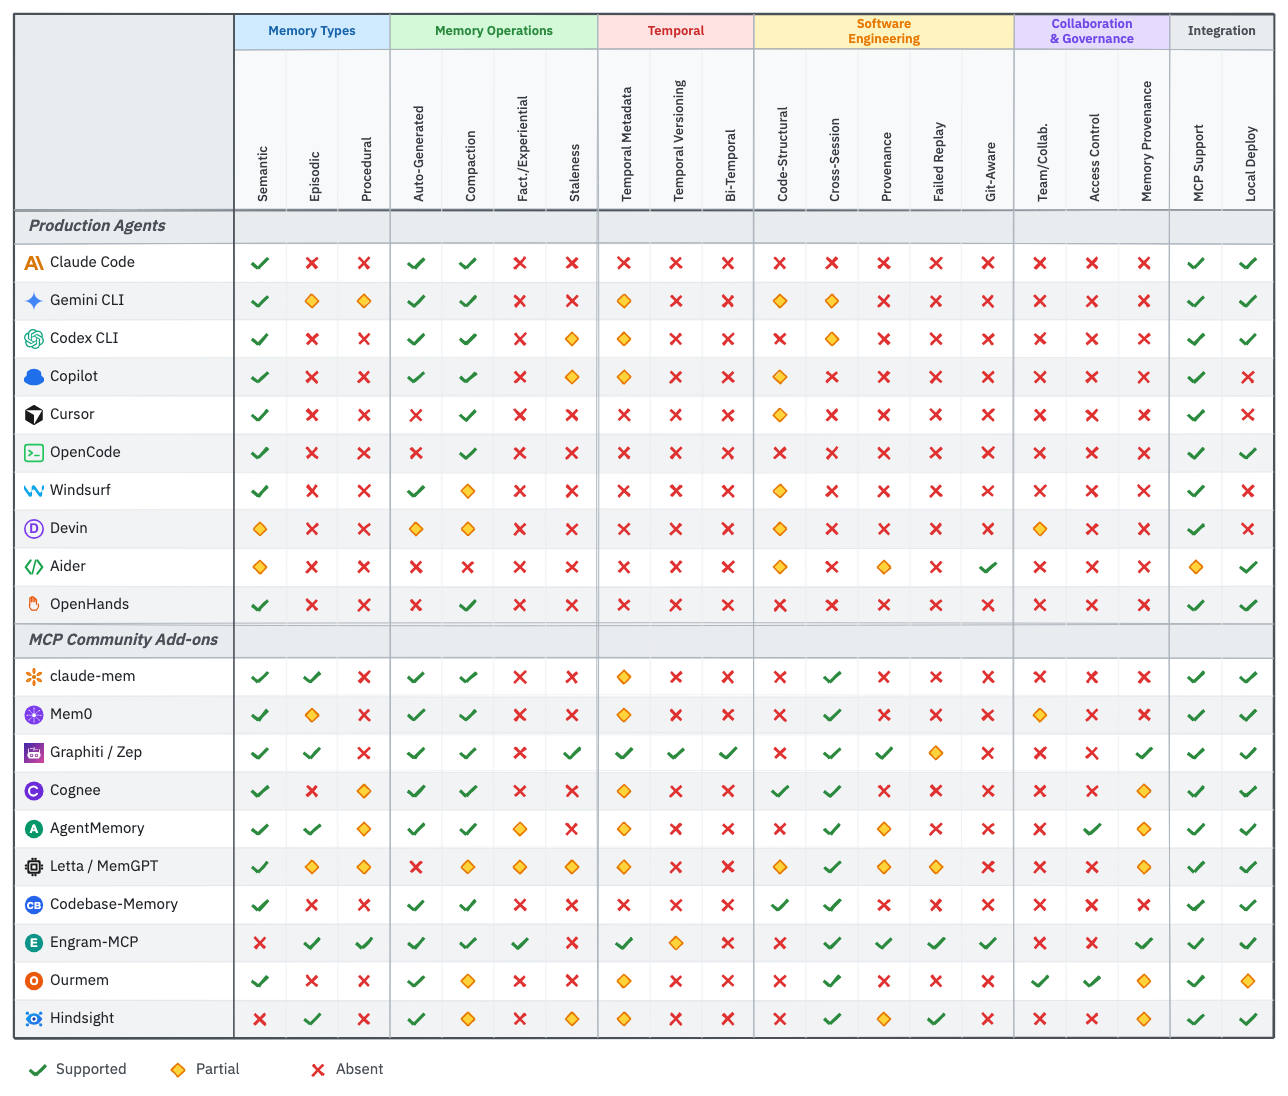
\includegraphics[width=0.92\textwidth]{ecosystem-table-expanded.png}
\end{frame}

%% ==========================================================================
%% SECTION 3 — Memory Architectures
%% ==========================================================================
\section{Memory Architectures}

\begin{frame}[plain]
  \sectionpage
\end{frame}

\begin{frame}{Three Paradigms}
  Classification of ICLR 2026 MemAgents workshop contributions:

  \vspace{0.3cm}

  \begin{columns}[T]
    \begin{column}{0.30\textwidth}
      \centering
      \textbf{\textcolor{pRed}{Extraction-Based}}\\[0.2cm]
      {\small Mem0\\[0.15cm]
      Extract atomic facts\\
      Vector-indexed retrieval\\[0.15cm]
      \alert{Excels at factual recall}\\
      Lossy by design}
    \end{column}

    \begin{column}{0.30\textwidth}
      \centering
      \textbf{\textcolor{pRed}{Self-Managing}}\\[0.2cm]
      {\small Letta / MemGPT\\[0.15cm]
      LLM manages its own memory\\
      Hierarchical read/write/search\\[0.15cm]
      \alert{Behavioral continuity}\\
      Less transparent}
    \end{column}

    \begin{column}{0.30\textwidth}
      \centering
      \textbf{\textcolor{pRed}{Graph-Based Temporal}}\\[0.2cm]
      {\small Graphiti / Zep\\[0.15cm]
      Bi-temporal validity intervals\\
      Event time vs.\ ingestion time\\[0.15cm]
      \alert{Causal reasoning}\\
      Added complexity}
    \end{column}
  \end{columns}

  \vspace{0.4cm}

  {\footnotesize Benchmarked head-to-head on LoCoMo-Plus cognitive memory evaluation (Gurawaliya et al., 2026)}
\end{frame}

\begin{frame}{The Case for Hybrid Architectures}
  \begin{itemize}
    \item LoCoMo-Plus results: \alert{no single paradigm masters all competency types}
    \item The three paradigms capture genuinely different aspects of memory
    \item Emerging directions:
    \begin{itemize}
      \item \textbf{RL-based management} (Memory-R1, AgeMem) --- learned policies discover
        non-obvious strategies, e.g.\ preemptive summarization
      \item \textbf{Multi-graph memory} (MAGMA) --- semantic, temporal, causal, entity
        graphs queried independently
      \item \textbf{Hierarchical consolidation} (TiMem) --- temporal memory tree
        for long execution traces
      \item \textbf{Hybrid local/cloud} (LightMem, HyMem) --- small models route,
        large models consolidate
    \end{itemize}
  \end{itemize}
\end{frame}

%% ==========================================================================
%% SECTION 4 — SE-Specific Mechanisms
%% ==========================================================================
\section{SE-Specific Mechanisms}

\begin{frame}[plain]
  \sectionpage
\end{frame}

\begin{frame}{Versioned Context \& Decision Provenance}
  \begin{columns}[T]
    \begin{column}{0.48\textwidth}
      \textbf{Intra-session:}
      \begin{itemize}
        \item \textbf{GCC} --- Git-inspired operations for agent working memory
        \item Branching, merging, rolling back context within a task
      \end{itemize}

      \vspace{0.3cm}

      \textbf{Inter-session:}
      \begin{itemize}
        \item \textbf{Lore} --- git commits as structured decision records
        \item Constraints, rejected alternatives, verification metadata via git trailers
      \end{itemize}
    \end{column}

    \begin{column}{0.48\textwidth}
      \textbf{Why it matters:}
      \begin{itemize}
        \item Each deviation in a mutating action \alert{reduces success odds}
        \item Errors grow as context length increases
        \item Agents drift from stale constraints: deprecated APIs, outdated conventions
        \item \alert{Decision provenance} lets agents understand \emph{why} before proposing changes
      \end{itemize}
    \end{column}
  \end{columns}
\end{frame}

\begin{frame}{Experiential \& Procedural Learning}
  \begin{itemize}
    \item \textbf{SWE Context Bench}: summarized experience improves resolution;
      \alert{unfiltered experience hurts}
    \item \textbf{Experiential Co-Learning} --- mine experiences from historical trajectories
    \item \textbf{ERL} --- reflect on trajectories $\rightarrow$ transferable heuristics;
      self-generated experiences outperform externally seeded ones
    \item \textbf{Live-SWE-agent} --- self-creates new tools during execution (procedural memory via self-modification)
    \item \textbf{Mem$^{\mathrm{p}}$} --- distills trajectories into step-by-step
      instructions + script-like abstractions
  \end{itemize}

  \vspace{0.3cm}

  \begin{alertblock}{Capacity Threshold}
    7B models do not benefit from experiential memory.
    32B+ models show pronounced gains. (WebCoach, 2026)
  \end{alertblock}
\end{frame}

\begin{frame}{Knowledge Graphs \& Collaboration}
  \begin{columns}[T]
    \begin{column}{0.48\textwidth}
      \textbf{Graph memory for SE:}
      \begin{itemize}
        \item \alert{Dependency tracking} --- files, imports, class hierarchies
        \item \alert{Decision provenance} --- ADRs, review discussions, commit rationale
        \item \alert{Temporal evolution} --- API validity, convention adoption, deprecation
      \end{itemize}

      \vspace{0.2cm}
      {\small GAM: hierarchical graph memory significantly outperforms extraction-based approaches}
    \end{column}

    \begin{column}{0.48\textwidth}
      \textbf{Collaborative memory:}
      \begin{itemize}
        \item Strong single-agent bias in current research
        \item \textbf{Private} memory (debugging notes) vs.\ \textbf{shared} memory (conventions, decisions)
        \item Security: MINJA shows shared-memory agents vulnerable to \alert{injection attacks}
        \item No SE-specific governance: repo permissions, review approvals, release cycles
      \end{itemize}
    \end{column}
  \end{columns}
\end{frame}

%% ==========================================================================
%% SECTION 5 — Open Gaps & Vision
%% ==========================================================================
\section{Open Gaps \& Vision}

\begin{frame}[plain]
  \sectionpage
\end{frame}

\begin{frame}{Six Open Gaps}
  \begin{enumerate}
    \item \textbf{Cross-session learning} --- resolution trajectories discarded after each session;
      no production harness integrates experiential transfer
    \item \textbf{Temporal knowledge validity} --- no SE-specific temporal memory;
      only one SE-specific temporal benchmark exists
    \item \textbf{Procedural memory} --- SE craft knowledge is overwhelmingly procedural,
      yet it is the rarest type in research and production
    \item \textbf{Collaborative memory} --- teams need shared decisions, private notes,
      and repository-aligned access control
    \item \textbf{Governance \& security} --- memory injection attacks, GDPR-compliant
      deletion entirely unaddressed
    \item \textbf{MCP orchestration} --- no layer decides which memory to consult when,
      resolves conflicts, or manages lifecycle across layers
  \end{enumerate}
\end{frame}

\begin{frame}{Key Takeaway}
  \begin{block}{The Central Argument}
    \alert{Persistent, temporally grounded memory} is the prerequisite for
    software engineering agents that learn alongside the teams they serve.
  \end{block}

  \vspace{0.4cm}

  \begin{itemize}
    \item The factual-to-cognitive gap across production architectures is confirmed by benchmarks
    \item The MCP ecosystem provides composable building blocks ---
      but assembling the full stack remains a manual integration challenge
    \item Closing these gaps requires transforming SE agents from\\
      \alert{amnesic tools} into \alert{learning collaborators}
  \end{itemize}

  \vspace{0.3cm}

  {\footnotesize Banf, Kuhn, Garcarz, Becker --- Perelyn GmbH, Munich}
\end{frame}

%% ==========================================================================
%% DISCUSSION
%% ==========================================================================

\begin{frame}{Discussion}
  \centering
  \vfill
  {\Large\bfseries Questions \& Discussion}
  \vfill

  \begin{itemize}
    \item How do you handle memory in your SE agent workflows today?
    \item Which memory type (episodic, procedural, temporal) would have
      the highest impact for your use case?
    \item Should memory governance be agent-managed or developer-controlled?
  \end{itemize}
  \vfill

  {\small michael.banf@perelyn.com}
\end{frame}

%% ==========================================================================
%% CLOSING SLIDE
%% ==========================================================================
\begin{frame}[plain]
  \titlepage
\end{frame}

\end{document}
